\mysection{}{Vorüberlegungen} \label{sec:Vorueberlegungen}

Um die Fragestellung realistisch umsetzen zu können ist es nötig, schon vorab Entscheidungen über Richtung und Umfang des Projekts zu treffen.

\subsection{Plugin-Umfang}
Es soll Entwicklern mit Uniplug möglich sein, ohne Kenntnis der nativen Programmierschnittstelle der jeweiligen 3D-Software, Plugins zu entwickeln. Hier könnten im Voraus Einschränkungen getroffen werden um die Entwicklung zu vereinfachen. Zum Beispiel wäre es möglich sich auf die Erzeugung von Geometrie zu beschränken.

\subsection{Plugin-Aufbau}
Vorab wurden zwei Ansätze für den Aufbau von Uniplug evaluiert. Außer der schon teilweise beschriebenen kompletten und am besten automatisierte Übersetzung der Programmierschnittstelle, gibt es noch die Möglichkeit nativ für die jeweilige Software ein Plugin zu entwickeln, das dann die zu übersetzende Schnittstelle zu Uniplug bildet und somit schon einen ersten Schritt zur Normalisierung und logischen Übersetzung bietet. Weitere Informationen zu den einzelnen Verfahren finden sich in \ref{sec:header}.

\subsection{Entscheidungen}
Die Entscheidung fiel auf eine möglichst vollständige Übersetzung ohne Zwischenschritt über ein Plugin. Dieser Ansatz bietet aber bei Erfolg einen wesentlich direkteren und auch komfortableren Zugriff auf Seiten von Uniplug, da jegliche logische Konvertierung im Rahmen von \CS direkt als Teil von Uniplug erfolgen kann.

\begin{figure}[htbp]
\center
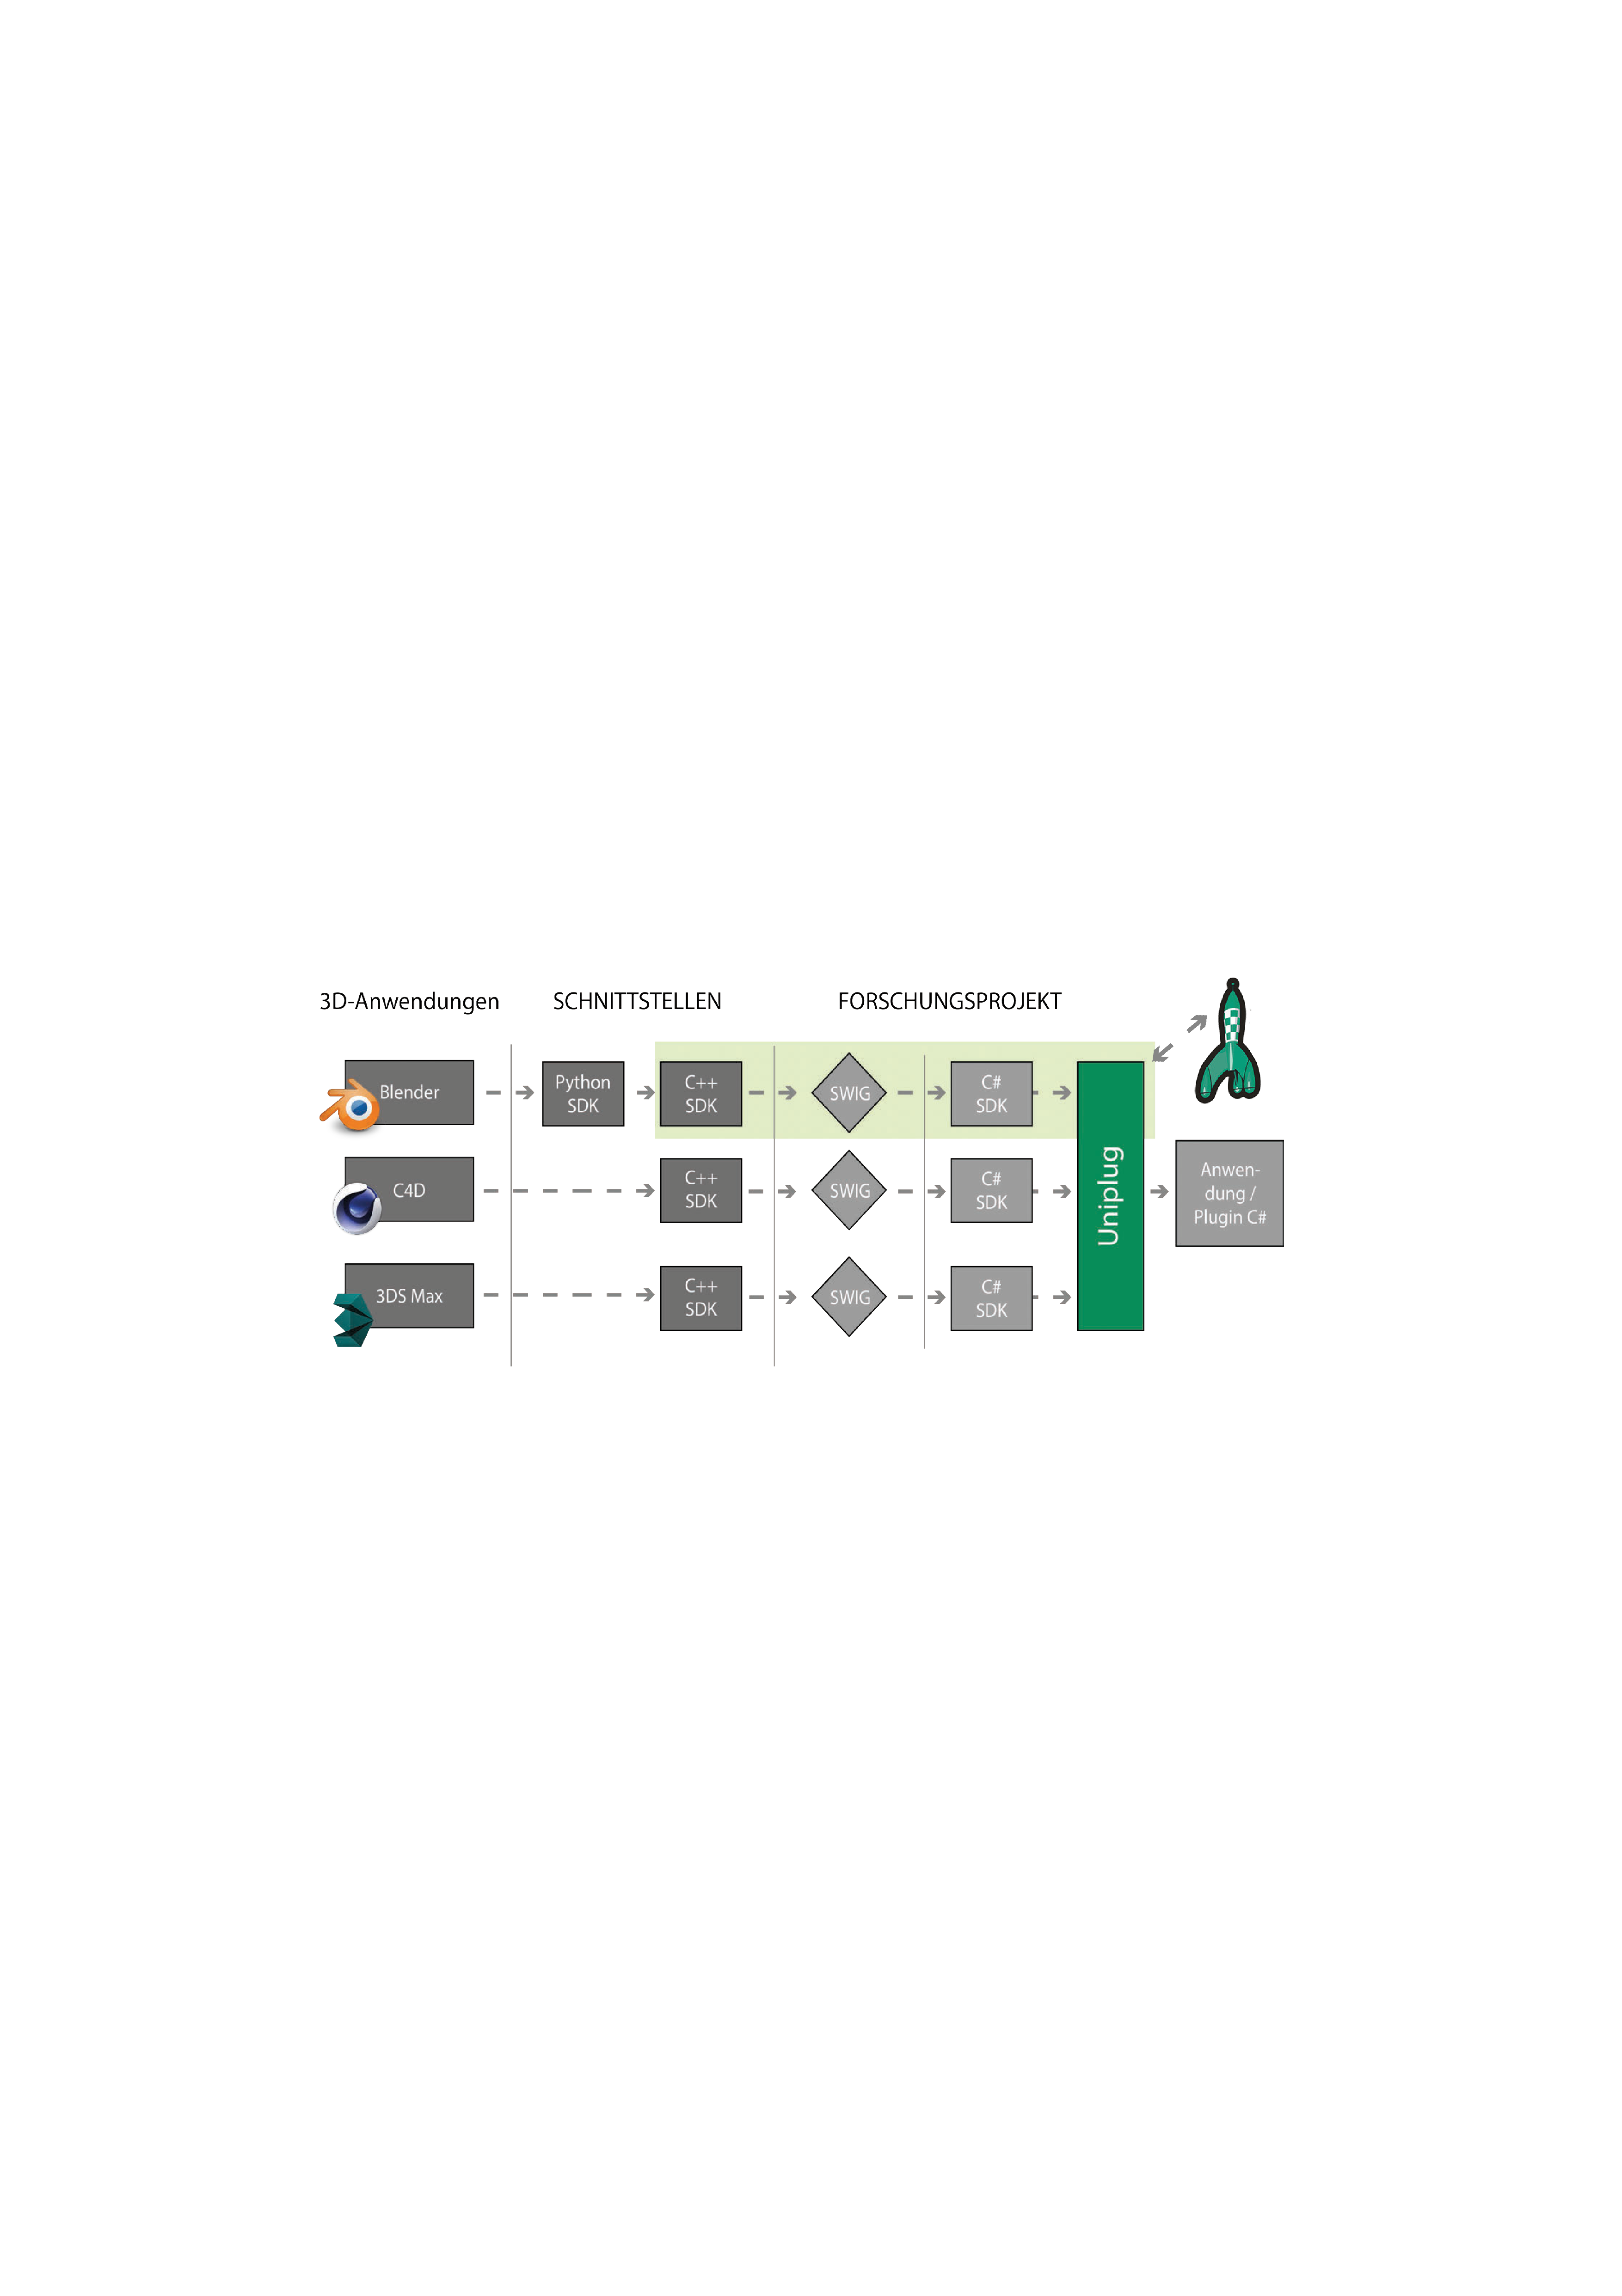
\includegraphics[width=1\textwidth]{images/aufbau}
\caption{Schematische Darstellung des Aufbaus}
\label{fig:aufbau}
\end{figure}